
\paragraph{The Eclipse Cloud Development project}
As mentioned in the introduction (\cref{sec:intro-eclipse-cloud}), the Eclipse ecosystem is interested in running software in the \gls{cloud}.
This means that they have spent the last few years creating tools to support \gls{cloud} oriented deployments for software built on \acrlong{EMF}.
The Eclipse Foundation has an umbrella project called \textit{Eclipse Cloud Development}.
In the Eclipse Foundation, a project is not a single codebase, but rather a home for frameworks, tools and components.
Under this umbrella exists projects like \textit{EMF.Cloud}, \textit{Eclipse Che}, \textit{Eclipse GLSP}, \textit{Eclipse Theia}, \textit{Eclipse OpenVSX} and more~\cite{beatonEclipseCloudDevelopment2014}.

\subsection{EMF.Cloud}
The Eclipse ecosystem found it suitable to create a new project under this umbrella, and called it \textit{Eclipse EMF.Cloud}.
The description for Eclipse EMF.Cloud starts with the following:
\begin{quote}
  ``\textit{Eclipse EMF.cloud comprises a set of components that facilitate and simplify the adoption of the Eclipse Modeling Framework (EMF) in cloud-based applications.\\
  \textelp{}\\
  As a consequence, by its nature, EMF.cloud is open to any software project that aims to address the challenges and specific requirements of using any aspect of EMF in a browser-based setting or cloud deployment.}''\\
  ---~\textcite{smithEclipseEMFCloud2019}
\end{quote}

\paragraph{EMF.Cloud software}
The components provided by EMF.Cloud are still in active development.
Most of them center around building a modeling environment in \gls{Theia}, for existing \acrshort{EMF} models.
The example case that is used is a ``Coffee brewing model''.
Because much of the work targets Theia, the Eclipse ecosystem uses Theia Extensions.
This means they can not be used in \gls{Gitpod}, because the \acrshort{IDE} has to be replaced with their customized Theia.
However, much of the work here is still relevant, as components to use in a \gls{VSCode} extension, and as design to draw inspiration from.\\

The EMF.Cloud project currently provides these components, according to \cite{tobiasortmayrEclipseemfcloudEmfcloud2021}:

\begin{itemize}
  \item modelserver
  \item modelserver-theia
  \item model-validation
  \item coffee.editor
  \item ecore-glsp
  \item theia-tree-editor
  \item json-forms-property-view
  \item modelserver-glsp-integration
  \item emf-jackson
\end{itemize}

The most relevant components for this thesis are detailed in the following subsections.

\subsubsection{Model Server}
The EMF.Cloud Model Server provides a web server for working with \acrshort{EMF} models.
While \acrshort{EMF} already support model loading, manipulation and serialization in the \acrshort{EMF} runtime \acrshort{API}, this server exposes these to the web.
It does so by providing a \gls{REST} \acrshort{API} for working with models, and \gls{WebSocket} channels for subscribing to change events.
The Model Server also manages a ``shared editing domain'' for the loaded models, and changes models using \acrshort{EMF} \texttt{Command}s~\cite{foundationEMFCloud}.\\

This Model Server is already used in other EMF.Cloud components, like the coffee editor and ecore-glsp~\cite{eugenneufeldEclipseemfcloudCoffeeeditor2021,ninadoschekEclipseemfcloudEcoreglsp2021}.

\subsubsection{Theia Tree Editor}\label{par:theia-tree-editor}
Theia Tree Editor is a framework for creating master-detail tree editors~\cite{foundationEMFCloud}.
It uses the Theia extension mechanism, and uses core components of \gls{Theia} itself~\cite{rekstadModelingEnvironmentCloud2020}.
This hinders reuse in other \acrshortpl{IDE} like \gls{VSCode}.
However, the data structures and configuration schemas used in the Theia Tree Editor are good sources for design inspiration.
A diagram of its \texttt{Node} interface (for tree nodes) is shown in \cref{fig:theia-tree-editor-nodes}\footnote{Node source code: \href{https://github.com/eclipse-emfcloud/theia-tree-editor/blob/3da9d6a3c58cad140c228408b92a554fe5dd1b41/theia-tree-editor/src/browser/interfaces.ts\#L30}{\nolinkurl{https://github.com/eclipse-emfcloud/theia-tree-editor/blob/3da9d6a3c58cad140c228408b92a554fe5dd1b41/theia-tree-editor/src/browser/interfaces.ts\#L30}}.}
\footnote{SelectableTreeNode source: \href{https://github.com/eclipse-theia/theia/blob/af9b883dd929c79c1593bf4bd526df11600e21cf/packages/core/src/browser/tree/tree-selection.ts\#L109}{\nolinkurl{https://github.com/eclipse-theia/theia/blob/af9b883dd929c79c1593bf4bd526df11600e21cf/packages/core/src/browser/tree/tree-selection.ts\#L109}}.}.


\begin{figure}[htbp]  % order of priority: h here, t top, b bottom, p page
  \centering
  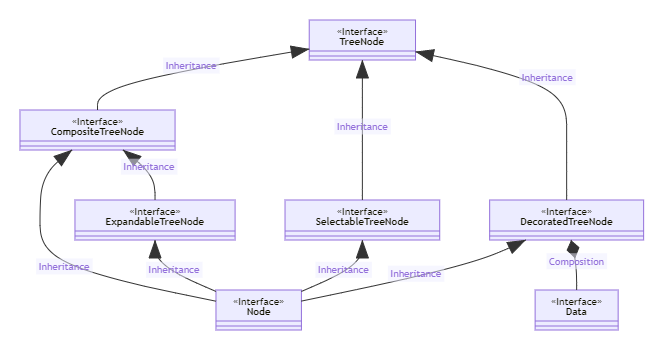
\includegraphics[width=\textwidth]{figures/pre-project/theia-tree-editor-node.png}
  \caption[Class Hierarchy of Theia Tree Editor Nodes]{A class hierarchy of the tree nodes in Theia Tree Editor. Class properties and methods are not shown. The \texttt{Node} interface extends several different interfaces, picking up various properties from each. Only the \texttt{Node} interface is in the Theia Tree Editor library itself. The other interfaces are in the core \gls{Theia} codebase. Adopted from ``Figure 2.7'' in \cite[p.~15]{rekstadModelingEnvironmentCloud2020}}\label{fig:theia-tree-editor-nodes}
\end{figure}

\subsubsection{Coffee Editor}
The Coffee Editor is an example application, trying to demonstrate the use of EMF.Cloud components in a real \gls{cloud} deployment.
This editor uses \gls{Theia}, JSON-Forms, \acrshort{GLSP}, a code generator, and the Model Server~\cite{foundationEMFCloud}.
This editor is interesting because it applies the technologies, demonstrating their use, purpose and value.
It also demonstrates the use of a Model Server shared among multiple editing components, like the GLSP and Theia Tree Editor working on the same backing coffee \acrshort{EMF} model instances.

\subsection{Graphical Language Server Platform (GLSP)}\label{sec:glsp}

This is another project under the Eclipse Cloud Development project.
The \acrfull{GLSP} is a framework for building diagram editors in the web.
The editors can either be standalone or integrated into \gls{Theia} and \gls{VSCode}.
The \acrshort{GLSP} defines its own \acrfull{LSP} for diagrams~\cite{eclipsefoundationGLSP2020}.
A figure from the official website is shown in \cref{fig:glsp-overview}.\\

This is a good source of design inspiration, because it both works with \acrshort{EMF} models, and it applies the \acrlong{LSP} architecture to a new domain other than text editing.

\begin{figure}[htbp]  % order of priority: h here, t top, b bottom, p page
  \centering
  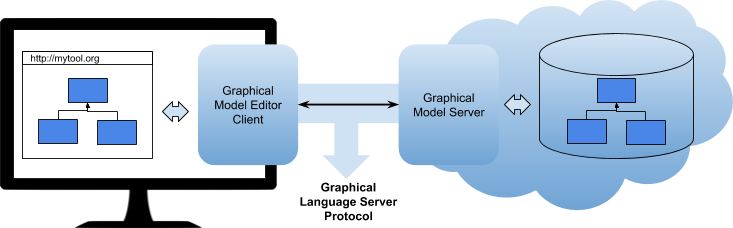
\includegraphics[width=\textwidth]{figures/pre-project/glsp-overview.png}
  \caption[GLSP Overview]{A diagram of GLSP. A web based diagram editor shows the diagram obtained from a Graphical Model Editor Client. This client talks to a graphical model server over the Graphical Language Server Protocol. Copied from \cite{eclipsefoundationGLSP2020}.}\label{fig:glsp-overview}
\end{figure}

\paragraph{GLSP Protocol}\label{par:glsp-actionmessage}
The \acrshort{LSP}-based protocol has a very small ``surface area''.
The protocol uses the same Base Protocol as defined in \acrshort{LSP} (see \cref{sec:lsp}).
The java implementation also uses the same libraries as Eclipse's Java \acrshort{LSP} server: the LSP4J jsonrpc library.
The server side of the GLSP protocol is shown in \cref{lst:glsp-server}.
Compare this to \acrshort{LSP}, which has about 40 Requests and 20 Notifications --- this GLSP protocol only has two requests and one Notification.
Instead of defining many different methods, the ``meat'' of the protocol is inside the \texttt{process} method.
The \texttt{ActionMessage} holds an \texttt{Action}, which is an abstract class with a \texttt{kind} field.
This \texttt{Action} is extended (subclassed) to about 20 different versions.
These have names like \texttt{FitToScreenAction}, \texttt{CenterAction}, \texttt{SelectAction}, \texttt{SaveModelAction}~\cite{tobiasortmayrEclipseglspGlspserverActions2021}.
The GLSP client and server implementations rely on \textit{action handlers}.
The Grphical Modeling Editor Client (usually inside \gls{VSCode} or \gls{Theia}) can decide if an \texttt{ActionMessage} from the diagram viewer should be forwarded to the Graphical Model Server or not.
Sometimes the action can be performed entirely inside the client.
The same applies for messages from the server, which can be forwarded to the diagram editor or stop in the Graphical Model Editor Client~\cite{tobiasortmayrEclipseglspGlspvscodeintegration2021}.

\begin{lstlisting}[language=java, label={lst:glsp-server}, caption={[GLSP Server Interface]GLSP Server java interface. Copied from \cite{philiplangerEclipseglspGlspserver2021}.}]
package org.eclipse.glsp.server.jsonrpc;

import java.util.concurrent.CompletableFuture;

import org.eclipse.glsp.server.actions.ActionMessage;
import org.eclipse.glsp.server.protocol.GLSPServer;
import org.eclipse.glsp.server.protocol.InitializeParameters;
import org.eclipse.lsp4j.jsonrpc.services.JsonNotification;
import org.eclipse.lsp4j.jsonrpc.services.JsonRequest;

public interface GLSPJsonrpcServer extends GLSPServer<GLSPJsonrpcClient> {
   @Override
   @JsonRequest
   CompletableFuture<Boolean> initialize(InitializeParameters params);

   @Override
   @JsonNotification
   void process(ActionMessage message);

   @Override
   @JsonRequest
   CompletableFuture<Boolean> shutdown();
}
\end{lstlisting}

\subsection{Other Tools by the Eclipse Ecosystem}
Not all the efforts by the Eclipse ecosystem are made under the Eclipse Foundation's management.
Some projects exist outside this, in code repositories belonging to individuals and organizations that work with \acrshort{EMF}.
Some of the most relevant software projects are described below.

\subsubsection{JSON-Forms}\label{sec:json-forms}

The purpose of JSON-Forms is to easily create user interfaces for data entry in the web, using HTML forms.
A screenshot of such a form is shown in \cref{fig:json-forms-example}.
JSON-Forms is a project by the EclipseSource organization.
This is the same organization that created the EMF Forms based \gls{Ecore} editor for \gls{Eclipse}, described in \cref{sec:emfforms-editor}.\\

JSON-Forms is using the same core approach as EMF Forms, where the view is described in a declarative fashion with a \textit{UI schema}.
This schema describes a data entry form.
It describes the input fields, their labels, what data they effect and the grouping of view elements~\cite{eclipsesourceWhatJSONForms}.\\

In addition to a UI schema, a form using JSON-Forms needs a \textit{JSON schema}, which describes the types, structure and validation rules for the underlying data.
Together, these two schemas are enough for JSON-Forms to render and edit a \gls{JSON} data object in a user interface.

\begin{figure}[htbp]  % order of priority: h here, t top, b bottom, p page
  \centering
  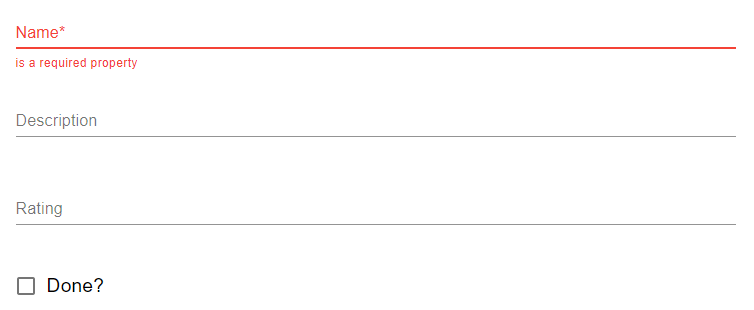
\includegraphics[width=\textwidth]{figures/pre-project/json-forms-example.png}
  \caption[JSON-Forms Example]{Example of a form rendered with JSON-Forms. Adopted from \cite{eclipsesourceWhatJSONForms}.}\label{fig:json-forms-example}
\end{figure}

\subsubsection{CrossEcore}
CrossEcore is a project by Simon Schwichtenberg with the aim of cross platform code generation using \acrshort{EMF}.
It targets the programming languages C\#, TypeScript, JavaScript, and Swift.
CrossEcore also implements the \acrshort{EMF} runtime \acrshort{API} for these languages, as well as an \gls{OCL} compiler~\cite{simonschwichtenbergCrossecoreEcoretypescript2021}.\\

This project is relevant because it can generate TypeScript code from \gls{Ecore} models, and has also experimented with creating online editors~\cite{simonschwichtenbergCrossEcore}.

\iffalse
% Not relevant enough
\subsubsection{ecore.js}
% TODO
* Under emfjson
\fi
